% Options for packages loaded elsewhere
\PassOptionsToPackage{unicode}{hyperref}
\PassOptionsToPackage{hyphens}{url}
%
\documentclass[
  13pt,
  ignorenonframetext,
]{beamer}
\usepackage{pgfpages}
\setbeamertemplate{caption}[numbered]
\setbeamertemplate{caption label separator}{: }
\setbeamercolor{caption name}{fg=normal text.fg}
\beamertemplatenavigationsymbolsempty
% Prevent slide breaks in the middle of a paragraph
\widowpenalties 1 10000
\raggedbottom
\setbeamertemplate{part page}{
  \centering
  \begin{beamercolorbox}[sep=16pt,center]{part title}
    \usebeamerfont{part title}\insertpart\par
  \end{beamercolorbox}
}
\setbeamertemplate{section page}{
  \centering
  \begin{beamercolorbox}[sep=12pt,center]{part title}
    \usebeamerfont{section title}\insertsection\par
  \end{beamercolorbox}
}
\setbeamertemplate{subsection page}{
  \centering
  \begin{beamercolorbox}[sep=8pt,center]{part title}
    \usebeamerfont{subsection title}\insertsubsection\par
  \end{beamercolorbox}
}
\AtBeginPart{
  \frame{\partpage}
}
\AtBeginSection{
  \ifbibliography
  \else
    \frame{\sectionpage}
  \fi
}
\AtBeginSubsection{
  \frame{\subsectionpage}
}
\usepackage{amsmath,amssymb}
\usepackage{lmodern}
\usepackage{iftex}
\ifPDFTeX
  \usepackage[T1]{fontenc}
  \usepackage[utf8]{inputenc}
  \usepackage{textcomp} % provide euro and other symbols
\else % if luatex or xetex
  \usepackage{unicode-math}
  \defaultfontfeatures{Scale=MatchLowercase}
  \defaultfontfeatures[\rmfamily]{Ligatures=TeX,Scale=1}
\fi
\usetheme[]{metropolis}
% Use upquote if available, for straight quotes in verbatim environments
\IfFileExists{upquote.sty}{\usepackage{upquote}}{}
\IfFileExists{microtype.sty}{% use microtype if available
  \usepackage[]{microtype}
  \UseMicrotypeSet[protrusion]{basicmath} % disable protrusion for tt fonts
}{}
\makeatletter
\@ifundefined{KOMAClassName}{% if non-KOMA class
  \IfFileExists{parskip.sty}{%
    \usepackage{parskip}
  }{% else
    \setlength{\parindent}{0pt}
    \setlength{\parskip}{6pt plus 2pt minus 1pt}}
}{% if KOMA class
  \KOMAoptions{parskip=half}}
\makeatother
\usepackage{xcolor}
\newif\ifbibliography
\usepackage{color}
\usepackage{fancyvrb}
\newcommand{\VerbBar}{|}
\newcommand{\VERB}{\Verb[commandchars=\\\{\}]}
\DefineVerbatimEnvironment{Highlighting}{Verbatim}{commandchars=\\\{\}}
% Add ',fontsize=\small' for more characters per line
\usepackage{framed}
\definecolor{shadecolor}{RGB}{248,248,248}
\newenvironment{Shaded}{\begin{snugshade}}{\end{snugshade}}
\newcommand{\AlertTok}[1]{\textcolor[rgb]{0.94,0.16,0.16}{#1}}
\newcommand{\AnnotationTok}[1]{\textcolor[rgb]{0.56,0.35,0.01}{\textbf{\textit{#1}}}}
\newcommand{\AttributeTok}[1]{\textcolor[rgb]{0.77,0.63,0.00}{#1}}
\newcommand{\BaseNTok}[1]{\textcolor[rgb]{0.00,0.00,0.81}{#1}}
\newcommand{\BuiltInTok}[1]{#1}
\newcommand{\CharTok}[1]{\textcolor[rgb]{0.31,0.60,0.02}{#1}}
\newcommand{\CommentTok}[1]{\textcolor[rgb]{0.56,0.35,0.01}{\textit{#1}}}
\newcommand{\CommentVarTok}[1]{\textcolor[rgb]{0.56,0.35,0.01}{\textbf{\textit{#1}}}}
\newcommand{\ConstantTok}[1]{\textcolor[rgb]{0.00,0.00,0.00}{#1}}
\newcommand{\ControlFlowTok}[1]{\textcolor[rgb]{0.13,0.29,0.53}{\textbf{#1}}}
\newcommand{\DataTypeTok}[1]{\textcolor[rgb]{0.13,0.29,0.53}{#1}}
\newcommand{\DecValTok}[1]{\textcolor[rgb]{0.00,0.00,0.81}{#1}}
\newcommand{\DocumentationTok}[1]{\textcolor[rgb]{0.56,0.35,0.01}{\textbf{\textit{#1}}}}
\newcommand{\ErrorTok}[1]{\textcolor[rgb]{0.64,0.00,0.00}{\textbf{#1}}}
\newcommand{\ExtensionTok}[1]{#1}
\newcommand{\FloatTok}[1]{\textcolor[rgb]{0.00,0.00,0.81}{#1}}
\newcommand{\FunctionTok}[1]{\textcolor[rgb]{0.00,0.00,0.00}{#1}}
\newcommand{\ImportTok}[1]{#1}
\newcommand{\InformationTok}[1]{\textcolor[rgb]{0.56,0.35,0.01}{\textbf{\textit{#1}}}}
\newcommand{\KeywordTok}[1]{\textcolor[rgb]{0.13,0.29,0.53}{\textbf{#1}}}
\newcommand{\NormalTok}[1]{#1}
\newcommand{\OperatorTok}[1]{\textcolor[rgb]{0.81,0.36,0.00}{\textbf{#1}}}
\newcommand{\OtherTok}[1]{\textcolor[rgb]{0.56,0.35,0.01}{#1}}
\newcommand{\PreprocessorTok}[1]{\textcolor[rgb]{0.56,0.35,0.01}{\textit{#1}}}
\newcommand{\RegionMarkerTok}[1]{#1}
\newcommand{\SpecialCharTok}[1]{\textcolor[rgb]{0.00,0.00,0.00}{#1}}
\newcommand{\SpecialStringTok}[1]{\textcolor[rgb]{0.31,0.60,0.02}{#1}}
\newcommand{\StringTok}[1]{\textcolor[rgb]{0.31,0.60,0.02}{#1}}
\newcommand{\VariableTok}[1]{\textcolor[rgb]{0.00,0.00,0.00}{#1}}
\newcommand{\VerbatimStringTok}[1]{\textcolor[rgb]{0.31,0.60,0.02}{#1}}
\newcommand{\WarningTok}[1]{\textcolor[rgb]{0.56,0.35,0.01}{\textbf{\textit{#1}}}}
\setlength{\emergencystretch}{3em} % prevent overfull lines
\providecommand{\tightlist}{%
  \setlength{\itemsep}{0pt}\setlength{\parskip}{0pt}}
\setcounter{secnumdepth}{-\maxdimen} % remove section numbering
\usepackage{MonashWhite}
\usepackage{amsmath,bm,booktabs,tikz,xcolor}
\usepackage{animate}

\setbeamercolor{description item}{fg=Orange}

\def\pred#1#2#3{\hat{#1}_{#2|#3}}
\def\damped{$_\text{d}$}
\def\h+{h_{m}^{+}}
\def\st#1{\rlap{#1}\textcolor{red}{\rule{1cm}{0.1cm}}}

\graphicspath{{figs/}}

% Monash title page
\setbeamerfont{title}{series=\bfseries,parent=structure,size={\fontsize{26}{30}}}
\setbeamertemplate{title page}
{
%\placefig{-0.01}{-0.01}{width=1.01\paperwidth,height=1.01\paperheight}{figs/MonashTitleSlide}
\begin{textblock}{7.5}(1,2)\fontsize{20}{30}\sf
{\raggedright\usebeamerfont{title}\par\inserttitle}
\end{textblock}
\begin{textblock}{7.5}(1,7.3)
{\raggedright{\insertauthor}\\[0.2cm]
\insertdate}
\end{textblock}}

\setlength\abovedisplayskip{0pt}

\AtBeginSection[] {
  \begin{frame}
  \frametitle{Outline}
    \tableofcontents[currentsection]
  \end{frame}
}

\usetikzlibrary{shapes,arrows}
\tikzstyle{decision} = [diamond, draw, fill=blue!20,
    text width=4.5em, text badly centered, node distance=4cm, inner sep=0pt]
\tikzstyle{block} = [rectangle, draw, fill=blue!20,
    text width=5cm, text centered, rounded corners, minimum height=4em]
\tikzstyle{line} = [draw, thick, -latex']
%\tikzstyle{line} = [->,thi
\tikzstyle{cloud} = [draw, ellipse,fill=red!20, node distance=3cm,
    minimum height=2em, text centered]
\tikzstyle{connector} = [->,thick]

\def\E{\text{E}}
\def\V{\text{Var}}
\def\up#1{\raisebox{-0.3cm}{#1}}

\setlength{\emergencystretch}{0em}
\setlength{\parskip}{0pt}
\def\fullwidth#1{\vspace*{-0.1cm}\par\centerline{\includegraphics[width=12.8cm]{#1}}}
\def\fullheight#1{\vspace*{-0.1cm}\par\centerline{\includegraphics[height=8.5cm]{#1}}}

\fontsize{13}{15}\sf
\usepackage[scale=0.85]{sourcecodepro}


\setbeamertemplate{navigation symbols}{}
\setbeamertemplate{footline}[]{}
\ifLuaTeX
  \usepackage{selnolig}  % disable illegal ligatures
\fi
\IfFileExists{bookmark.sty}{\usepackage{bookmark}}{\usepackage{hyperref}}
\IfFileExists{xurl.sty}{\usepackage{xurl}}{} % add URL line breaks if available
\urlstyle{same} % disable monospaced font for URLs
\hypersetup{
  pdftitle={Inference about the bias of a coin},
  pdfauthor={Giorgio Corani},
  hidelinks,
  pdfcreator={LaTeX via pandoc}}

\title{Inference about the bias of a coin}
\author{Giorgio Corani}
\date{Bayesian Data Analysis and Probabilistic Programming}

\begin{document}
\frame{\titlepage}

\begin{frame}[fragile]{References}
\protect\hypertarget{references}{}
\begin{itemize}
\tightlist
\item
  Kruschke
\item
  The Beta-Binomial model: Ch. 3 of
  \texttt{Bayes\ Rules!\ An\ Introduction\ to\ Applied\ Bayesian\ Modeling}

  \begin{itemize}
  \tightlist
  \item
    \url{https://www.bayesrulesbook.com/chapter-3.html\#chapter-3}
  \item
    Alicia A. Johnson, Miles Q. Ott, Mine Dogucu
  \end{itemize}
\end{itemize}
\end{frame}

\begin{frame}{Estimating the bias \(\theta\) of a coin}
\protect\hypertarget{estimating-the-bias-theta-of-a-coin}{}
\begin{itemize}
\tightlist
\item
  A coin falls tails with probability \(\theta \in [0,1]\)
\item
  \(\theta\) is the \emph{bias} of the coin

  \begin{itemize}
  \tightlist
  \item
    \(\theta\) =0: it always lands tails
  \item
    \(\theta\) =1: it always lands heads
  \end{itemize}
\item
  We flip the coin \(n\) times and we measure the number of heads \(y\).
\item
  Which is the posterior distribution \(p(\theta \mid y)\)?
\end{itemize}
\end{frame}

\begin{frame}{The coin problem}
\protect\hypertarget{the-coin-problem}{}
\begin{itemize}
\tightlist
\item
  The coin stands in for many real-world applications, such as
  estimating the success probability of a drug, the proportion of
  supporters of a political party or the click-through rate of an online
  advertisement.
\end{itemize}

\textbf{Assumptions}

\begin{itemize}
\tightlist
\item
  Each observation takes a binary value (head or tail; also referred to
  as \emph{success} and \emph{insuccess})
\item
  The \emph{success} usually refer to the rarer event among the two.
\item
  The flips are independent: the probability of \emph{heads} at the next
  flip does not depend on the outcome of the previous flips.
\item
  \(\theta\) is constant in all flips.
\end{itemize}
\end{frame}

\begin{frame}{The coin problem}
\protect\hypertarget{the-coin-problem-1}{}
A single flip takes:

\begin{itemize}
\item
  \emph{heads} with probability \(\theta\)
\item
  \emph{tails} with probability \(1-\theta\)
\item
  Assuming a constant \(\theta\) and the independence of the flips, the
  probability of the sequence: \[H \quad T  \quad T \quad H \quad H\]
\item
  is
  \[ \theta (1-\theta) (1-\theta) \theta \theta = \theta^2 (1-\theta)^3\]
\item
  The probability of \(y\) heads in \(n\) flips is:
  \[\theta^y (1-\theta)^{n-y}\]
\end{itemize}
\end{frame}

\begin{frame}{Binomial likelihood}
\protect\hypertarget{binomial-likelihood}{}
\[p(y \mid \theta) = \theta^y (1 − \theta)^{1−y}\] * This is probability
of the observing \(y\) tails within \(n\) flips, given a fixed value of
\(\theta\). * This a \emph{likelihood} function if we: * keep the
observation \(y\) fixed * the above probability is a function of
\(\theta\). * The likelihood function shows how the probability of the
observed data varies with \(\theta\).
\end{frame}

\begin{frame}{The Beta prior}
\protect\hypertarget{the-beta-prior}{}
\begin{itemize}
\tightlist
\item
  We need a continuous prior probability model for \(\theta\), i.e., a
  probability density function (pdf).
\item
  It specifies all possible values of \(\theta\) and the relative
  plausibility of each.

  \begin{itemize}
  \tightlist
  \item
    What values can \(\theta\) take and which are more plausible than
    others?
  \item
    Accounting for all possible outcomes of \(\theta\), the pdf
    integrates to or has an area of 1, much like a discrete pmf sums to
    1.
  \end{itemize}
\end{itemize}
\end{frame}

\begin{frame}{The Beta prior}
\protect\hypertarget{the-beta-prior-1}{}
\begin{itemize}
\tightlist
\item
  It is possible that \(f(\theta)>1\), thus a continuous pdf cannot be
  interpreted as a probability.
\item
  Probabilities are obtained by integrating the pdf, i.e.: \[
  P(c<\theta<d)=\int_c^d f(\theta) d\theta 
  \]
\end{itemize}
\end{frame}

\begin{frame}{The prior \(p(\theta)\)}
\protect\hypertarget{the-prior-ptheta}{}
\begin{itemize}
\item
  We need to define the prior probability of each value of \(\theta\) in
  \([0, 1]\).
\item
  The beta distribution, denoted by \(\text{Beta}(a, b)\), is a suitable
  prior for variables restricted to the \([0, 1]\) interval.
\item
  The density function is:
\end{itemize}

\begin{align*}
p(\theta) & = 
\frac{1} {\underbrace{B(a,b)}_{\text{normalizing constant}}}   
\theta^{a-1}(1-\theta)^ {b-1}
\propto \theta^{a-1}(1-\theta)^ {b-1} \qquad \qquad a,b>0 
\end{align*}

\begin{itemize}
\tightlist
\item
  Let us ignore the normalizing constant.
\end{itemize}

Note that:

\begin{itemize}
\tightlist
\item
  \(\theta\) is raised to the power of \(a−1\) (not \(a\))
\item
  \(1-\theta\) is raised to the power of \(b−1\) (not \(b\))
\end{itemize}
\end{frame}

\begin{frame}{Beta distribution}
\protect\hypertarget{beta-distribution}{}
\begin{itemize}
\item
  Expectation (i.e., mean): \[E(\theta)= \frac{a}{a+b} \]
\item
  Variance: \[\operatorname{VAR}(\theta)= \frac{ab}{(a+b)^2(a+b+1)} \]
\item
  Higher \(a\): the bulk of the distribution moves rightward
\item
  Higher \(b\): the bulk of the distribution moves leftward
\item
  Higher \(a\) and \(b\): the distribution gets more concentrated.
\end{itemize}
\end{frame}

\begin{frame}{Beta distribution with \(a = b = 1\)}
\protect\hypertarget{beta-distribution-with-a-b-1}{}
\begin{align*}
p(\theta) & \propto \theta^{a-1}(1-\theta)^ {b-1} \\
& =   \theta^{0}(1-\theta)^ {0} \\
& = 1
\end{align*}

\begin{itemize}
\tightlist
\item
  This a \emph{uniform} distribution: all values in \((0,1)\) are
  equally probable.
\item
  \(E(\theta)=\frac{a}{a+b} = 0.5\).
\end{itemize}

\begin{center}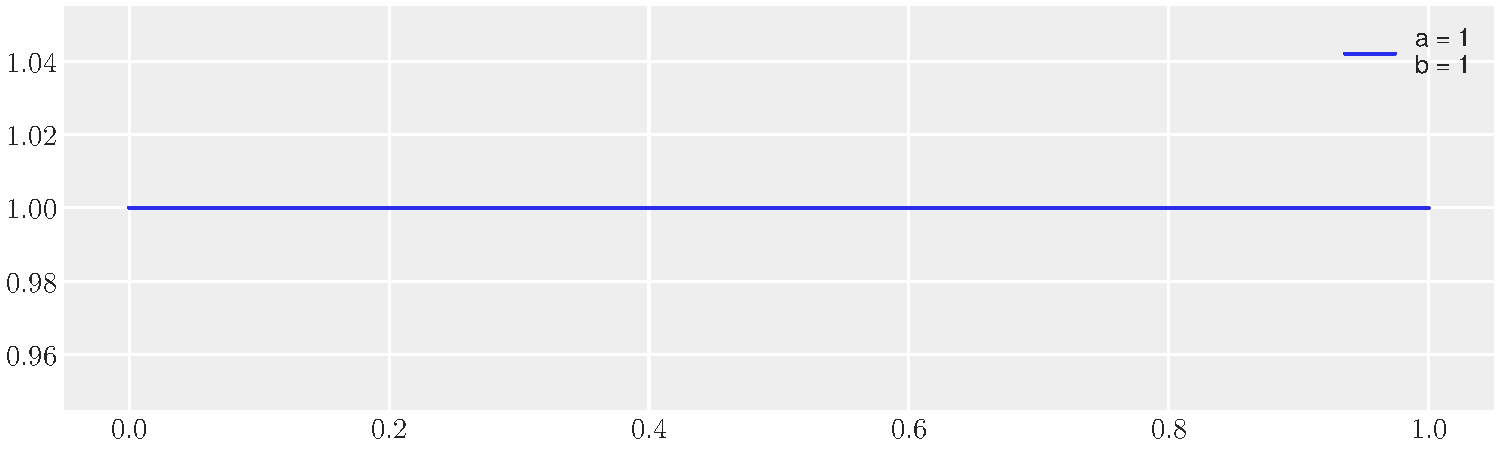
\includegraphics{3-coinTossing_files/figure-beamer/unnamed-chunk-2-1} \end{center}
\end{frame}

\begin{frame}{Increasing \(a\) and \(b\) the prior becomes more
concentrated}
\protect\hypertarget{increasing-a-and-b-the-prior-becomes-more-concentrated}{}
\begin{itemize}
\item
  If we increase \(a\) and \(b\) together, the prior becomes more
  concentrated around the expected value \(\theta=0.5\)
\item
  We can thus represent more confident beliefs about the coin being fair
\end{itemize}

\begin{center}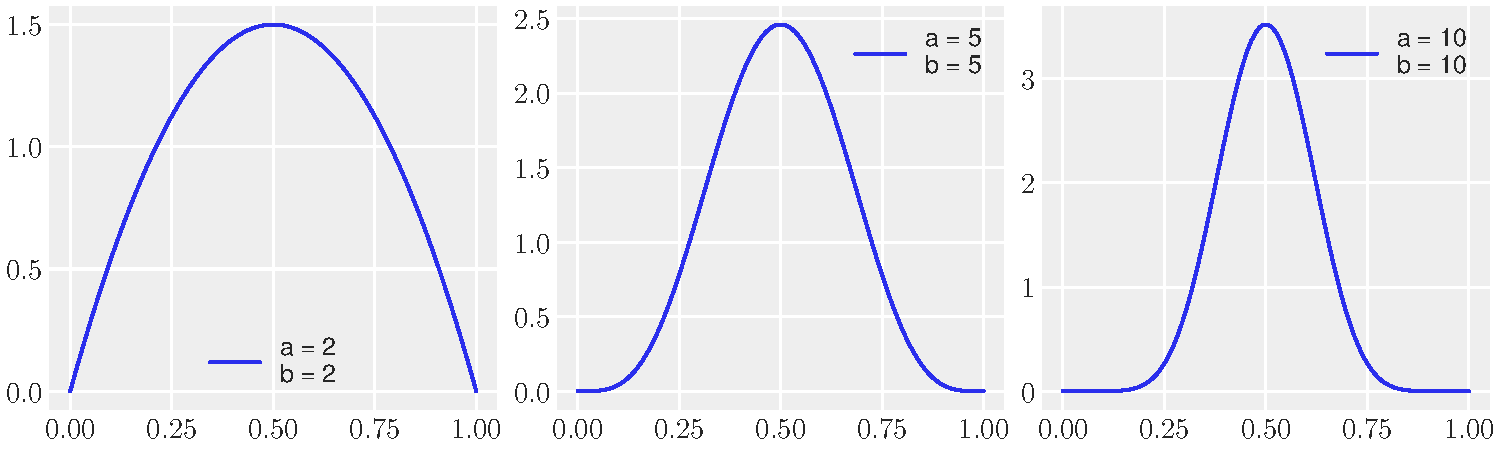
\includegraphics{3-coinTossing_files/figure-beamer/unnamed-chunk-3-3} \end{center}
\end{frame}

\begin{frame}{If we think the coin is rigged towards \emph{tails}}
\protect\hypertarget{if-we-think-the-coin-is-rigged-towards-tails}{}
\begin{itemize}
\item
  If we suspect the coin to be 70\% rigged towards heads, we set
  \(a=\frac{7}{3}b\).
\item
  We represent more confidence in this statement by:

  \begin{itemize}
  \tightlist
  \item
    increasing \(b\)
  \item
    keeping \(a=\frac{7}{3}b\).
  \end{itemize}
\end{itemize}

\begin{center}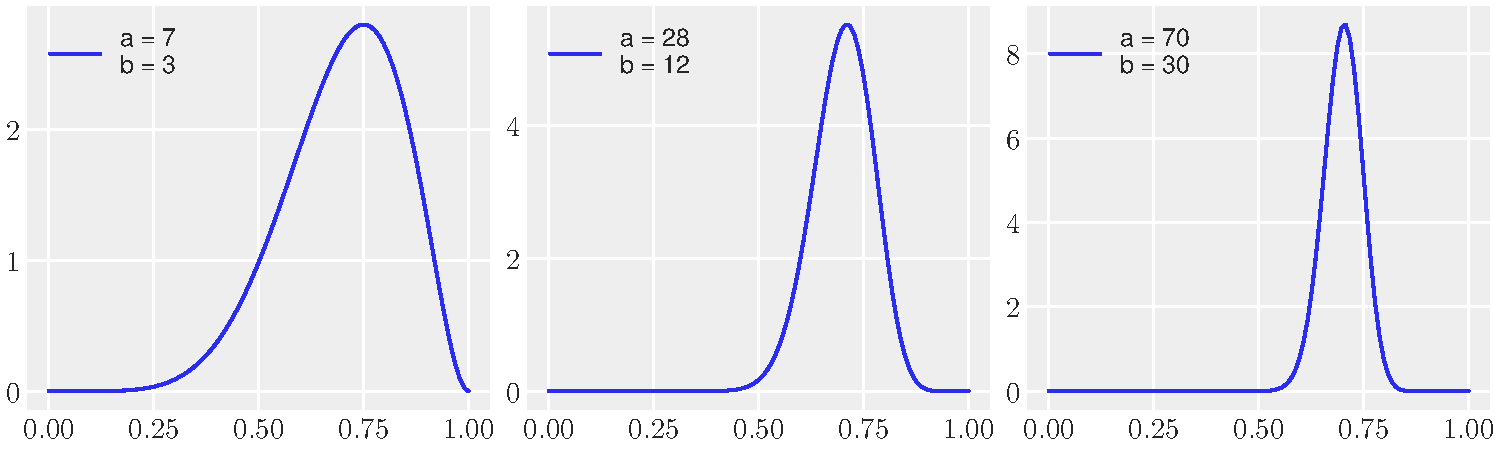
\includegraphics{3-coinTossing_files/figure-beamer/unnamed-chunk-4-5} \end{center}
\end{frame}

\begin{frame}[fragile]{Choice of \(a\) and \(b\)}
\protect\hypertarget{choice-of-a-and-b}{}
\begin{itemize}
\tightlist
\item
  The choice of \(a\) and \(b\) can be fine-tuned if you have an idea
  about the quantiles of your prior beliefs, not only the expected
  value.
\item
  This is how the 10-the and the 90-th percentile vary with \(a\) and
  \(b\):
\end{itemize}

\begin{Shaded}
\begin{Highlighting}[]
\ControlFlowTok{for}\NormalTok{ (a, b) }\KeywordTok{in}\NormalTok{  [(}\DecValTok{7}\NormalTok{, }\DecValTok{3}\NormalTok{), (}\DecValTok{28}\NormalTok{, }\DecValTok{12}\NormalTok{), (}\DecValTok{70}\NormalTok{, }\DecValTok{30}\NormalTok{)]:}
\NormalTok{    quantiles}\OperatorTok{=}\NormalTok{[}\FloatTok{0.10}\NormalTok{, }\FloatTok{0.90}\NormalTok{]}
\NormalTok{    q }\OperatorTok{=}\NormalTok{ beta.ppf(quantiles, a}\OperatorTok{=}\NormalTok{a, b}\OperatorTok{=}\NormalTok{b)}
    \BuiltInTok{print}\NormalTok{(}\StringTok{"a="}\NormalTok{, a , }\StringTok{" b="}\NormalTok{, b, }\StringTok{", q10="}\NormalTok{, q[}\DecValTok{0}\NormalTok{], }\StringTok{", q90="}\NormalTok{, q[}\DecValTok{1}\NormalTok{])}
\end{Highlighting}
\end{Shaded}

\begin{verbatim}
## a= 7  b= 3 , q10= 0.509918805554197 , q90= 0.8705027031423103
## a= 28  b= 12 , q10= 0.6055722379370202 , q90= 0.7899920979991506
## a= 70  b= 30 , q10= 0.6405652590000159 , q90= 0.757697282894839
\end{verbatim}
\end{frame}

\begin{frame}{We suspect the coin to be rigged but we do not in which
direction}
\protect\hypertarget{we-suspect-the-coin-to-be-rigged-but-we-do-not-in-which-direction}{}
\begin{itemize}
\tightlist
\item
  \(a<1, b<1\) yield a convex distribution
\item
  As they get closer to 0, the distribution becomes even more convex: we
  are now modelling the opinion that the coin is unlikely to be fair
\end{itemize}

\begin{center}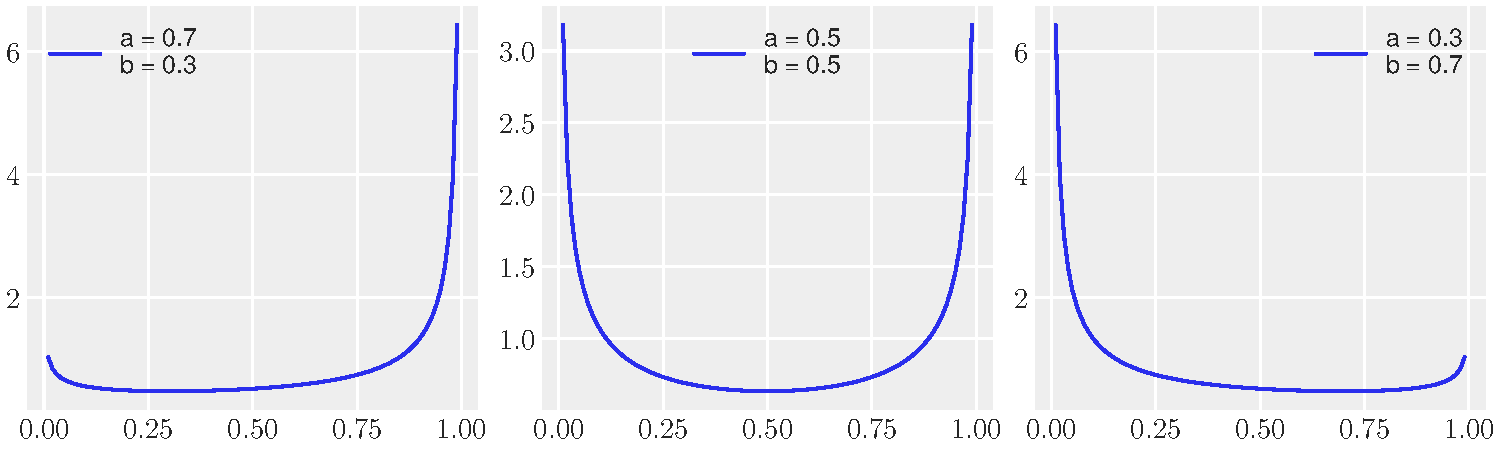
\includegraphics{3-coinTossing_files/figure-beamer/unnamed-chunk-6-7} \end{center}
\end{frame}

\begin{frame}{Discussion}
\protect\hypertarget{discussion}{}
The beta distribution can represent different types of prior beliefs\\
about \(\theta\), such as:

\begin{itemize}
\tightlist
\item
  all values of \(\theta\) are equally probable a priori
\item
  we think the coin is likely to be fair, but we are not fully sure
  (bell centered in \(\theta\)=0.5).
\item
  we think the coin is likely to be rigged towards tails (asymmetric
  distribution centered in e.g.~\(\theta\)=0.7, less or more
  concentrated).
\item
  we think the coin to be rigged, but she does not know in which way
  (convex distribution).
\end{itemize}
\end{frame}

\begin{frame}{Posterior}
\protect\hypertarget{posterior}{}
Adopting a beta prior for \(\theta\) and a binomial distribution as
\emph{likelihood}, we obtain a beta \emph{posterior} distribution with
updated parameters:

\begin{align*}
p(\theta) & \propto \theta^{a-1} (1-\theta)^{b}\\
p(y \mid \theta) & = \theta^{y} (1-\theta)^{n-y} \\
p(\theta \mid y) & \propto  \theta^{y+a-1} (1-\theta)^{n-y+b-1}\\
\end{align*}

The beta prior is \emph{conjugate} with the binomial likelihood, as we
obtain a beta posterior.
\end{frame}

\begin{frame}{Conjugacy}
\protect\hypertarget{conjugacy}{}
According to Bayes' theorem, the posterior is the product of the
likelihood and the prior: \[
p(\theta \mid y) \propto p(y \mid \theta) p(\theta)
\] In our case:

\begin{align*}
p(\theta \mid y) & \propto \theta^y (1-\theta)^{n-y}
\theta^{a-1} (1-\theta)^{b-1}\\
p(\theta \mid y) & \propto \theta^{y+a-1} (1-\theta)^{n-y+b-1}
\end{align*}

which is a Beta distribution (without expressing the normalization
constant).
\end{frame}

\begin{frame}{The posterior is a compromise of prior and likelihood}
\protect\hypertarget{the-posterior-is-a-compromise-of-prior-and-likelihood}{}
\begin{itemize}
\item
  Given the prior Beta(\(a\),\(b\)), the prior mean of \(\theta\) is:
  \[\frac{a}{a+b}\]
\item
  Having observed \(y\) tails in \(n\) flips, the posterior distribution
  of \(\theta\) is Beta(\(y+a\),\(n-y+b\)). The posterior mean is:
  \[E_{\text{post}}[\theta]=\frac{a + y}{a + y + b + n - y} = \frac{a + y}{a+ b + n} \]
\item
  Rearranging: \[ 
  \underbrace{\frac{a + y}{a+ b + n}}_{\text{posterior}} = 
  \underbrace{\frac{y}{n}}_{\text{observed proportion}}
  \underbrace{\frac{n}{n+a+b}}_{\text{weight}} + 
  \underbrace{\frac{a}{a+b}}_{\text{prior mean of $\theta$}}
  \underbrace{\frac{a+b}{n+a+b}}_{\text{weight of the prior}}  
  \]
\item
  The posterior mean is a weighted average of the prior mean and the
  observed proportion.
\item
  The weight of the observed proportion increases with \(n\); the weight
  of the prior mean increases with \(a\) and \(b\).
\end{itemize}
\end{frame}

\begin{frame}{Conjugacy}
\protect\hypertarget{conjugacy-1}{}
\begin{itemize}
\item
  If for a certain \emph{likelihood} the functional form of the \emph{a
  priori} and that of the \emph{a posteriori} coincide, it is said that
  the \emph{a priori} is conjugated with the \emph{likelihood}.
\item
  Historically, problems in Bayesian statistics were restricted to the
  use of conjugate priors, because of mathematical tractability.
\item
  However modern computational techniques allow obtaining posteriors
  even when conjugacy does not hold, allowing the resurgence of Bayesian
  statistics in recent years.
\end{itemize}
\end{frame}

\begin{frame}{Representing the Beta-binomial model}
\protect\hypertarget{representing-the-beta-binomial-model}{}
We represent the model as: \begin{align*}
\theta & \sim \operatorname{Beta}(a,b)\\
y & \sim \operatorname{Bin}(n,\theta)
\end{align*}

The symbol \(\sim\) shows the distribution followed by a certain
variable.
\end{frame}

\begin{frame}{Kruschke diagram of the beta binomial model}
\protect\hypertarget{kruschke-diagram-of-the-beta-binomial-model}{}
\begin{itemize}
\tightlist
\item
  In the top level we show the prior, below the likelihood, and finally
  the data.
\end{itemize}

\begin{center}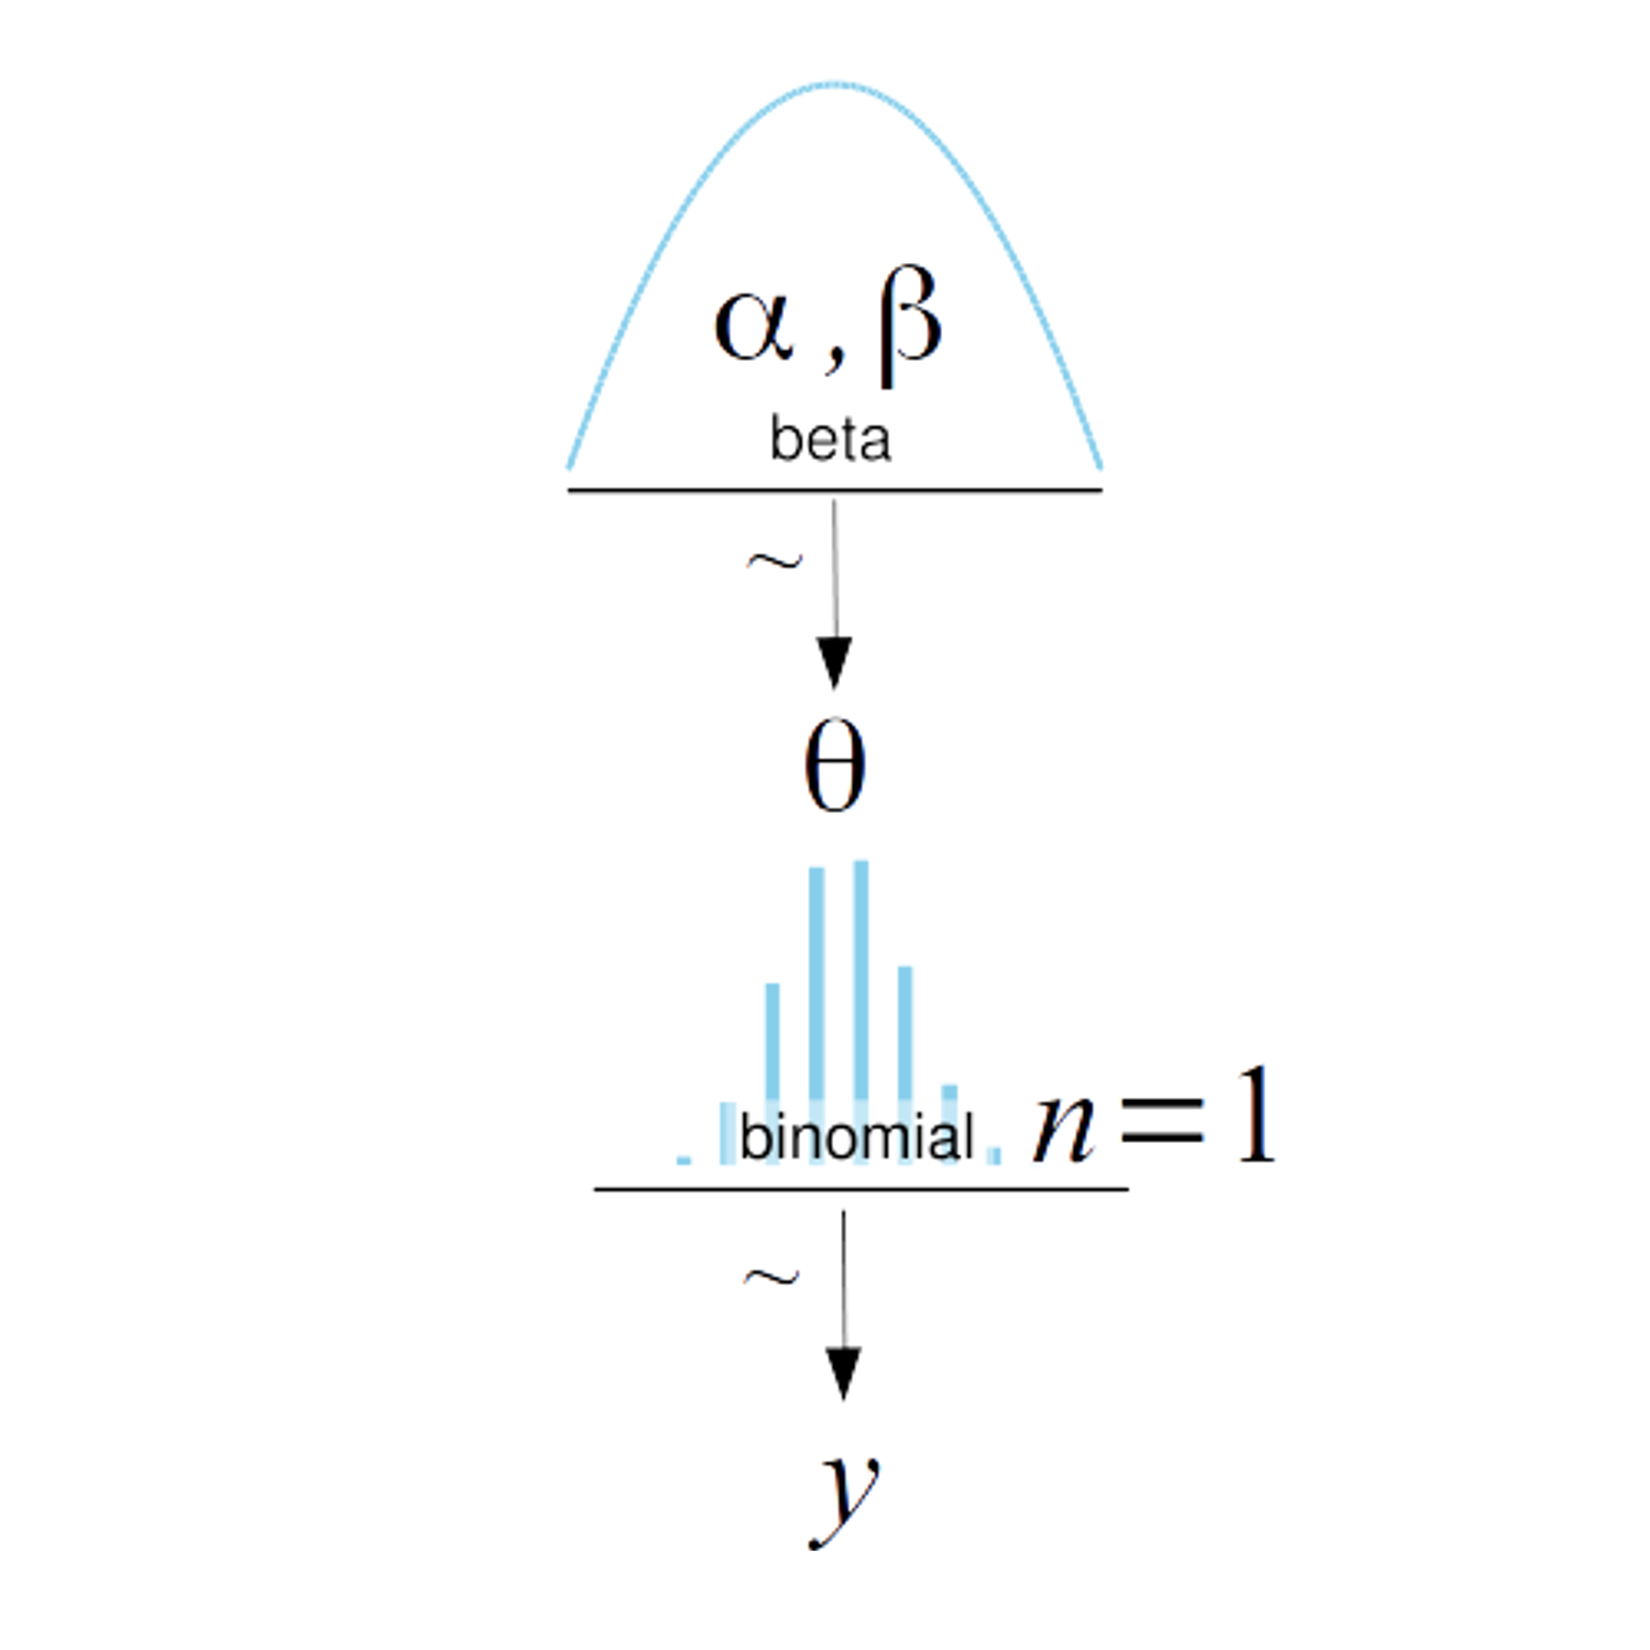
\includegraphics[width=22.92in]{coin_model} \end{center}
\end{frame}

\begin{frame}{Exercise: grid sampling (DISCUTERE CON MARCO)}
\protect\hypertarget{exercise-grid-sampling-discutere-con-marco}{}
\begin{itemize}
\tightlist
\item
  Choose a value of \(\theta\) and simulate 1000 Bernoulli trials from
  it; collect the value of \(n\) and \(y\)
\item
  Define your prior by setting \(a\) and \(b\) (do not abuse the fact
  that you know \(\theta\))
\item
  Discretize the values of \(\theta \in (0,1)\) by 0.01
\item
  Compute for each value of \(\theta\) the unnormalized posterior
  \$p(\theta \textbar{} mid y) \propto Beta(\theta;a,b) p(y \mid \theta)
  \$
\item
  Check the following:

  \begin{itemize}
  \tightlist
  \item
    given the large sample size, your posterior remains practically the
    same if you change the prior
  \item
    given to the large sample size, your posterior is concentrated
    around the true values of \(\theta\)
  \item
    your posterior is practically equivalent to
    \(Beta(\theta;a+y,b+n-y)\) also for small sample size.
  \end{itemize}
\end{itemize}
\end{frame}

\begin{frame}{CODE TO BE IMPLEMENTED}
\protect\hypertarget{code-to-be-implemented}{}
\end{frame}

\begin{frame}{Computation}
\protect\hypertarget{computation}{}
\begin{itemize}
\item
  In the course we will see how to use computational methods to compute
  the posteriori even with non-conjugate priors.
\item
  In the following we exploit conjugacy in order to explor the
  sensitivity of the posterior on the prior.
\end{itemize}
\end{frame}

\begin{frame}{Impact of the prior on the posterior}
\protect\hypertarget{impact-of-the-prior-on-the-posterior}{}
\begin{itemize}
\item
  We can start from different priors depending on subjective beliefs
  (priors might be used to encode domain expertise, and different
  experts would provide you with reasonable but different assessment)
\item
  Let us consider different priors
\end{itemize}

\begin{center}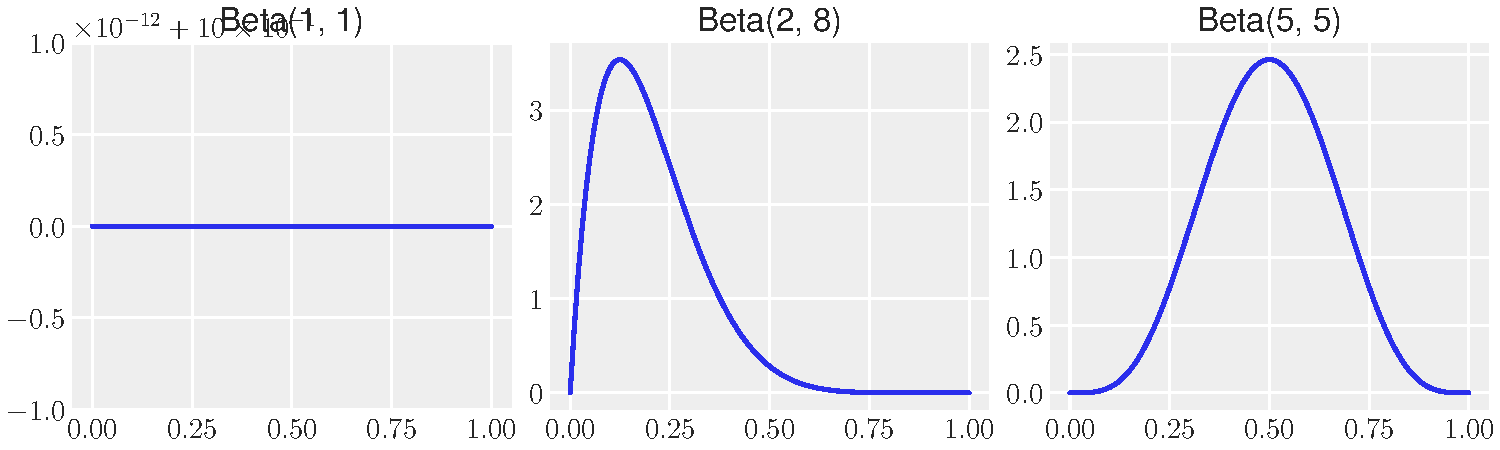
\includegraphics{3-coinTossing_files/figure-beamer/unnamed-chunk-8-1} \end{center}
\end{frame}

\begin{frame}[fragile]{The posterior depends on the priors when
observations are few (\(y\)=1 tails, \(n\)=2, heads=1)}
\protect\hypertarget{the-posterior-depends-on-the-priors-when-observations-are-few-y1-tails-n2-heads1}{}
\begin{center}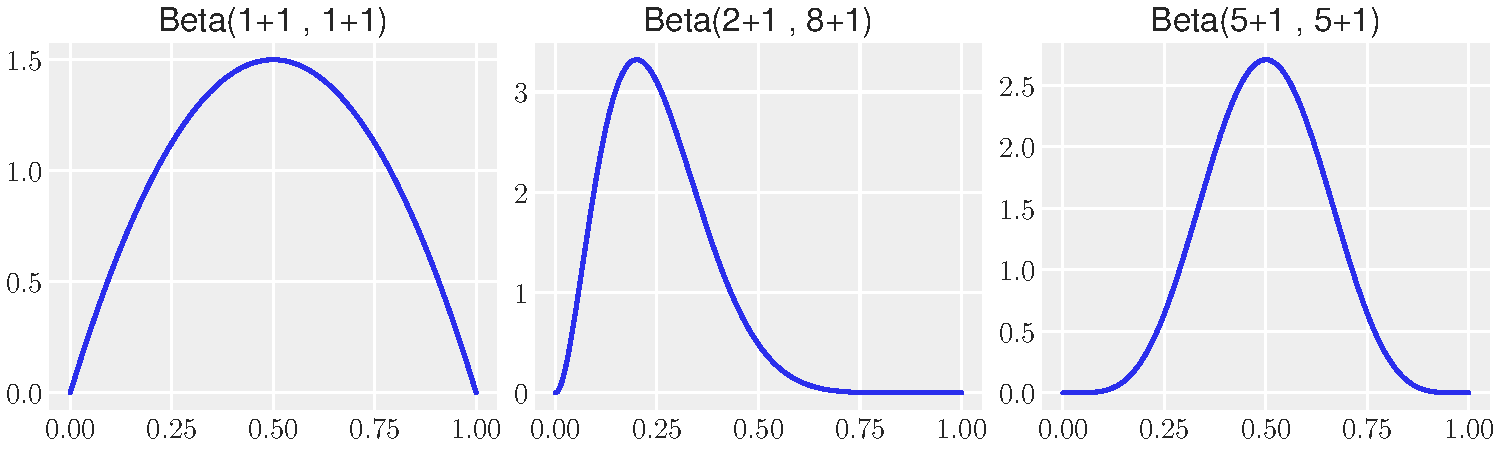
\includegraphics{3-coinTossing_files/figure-beamer/unnamed-chunk-9-3} \end{center}

\begin{itemize}
\tightlist
\item
  The Beta(2,8) represents the following beliefs:

  \begin{itemize}
  \tightlist
  \item
    expected value = \(\frac{2}{2+8}=0.2\)
  \item
  \end{itemize}
\end{itemize}

\begin{Shaded}
\begin{Highlighting}[]
\ImportTok{from}\NormalTok{ scipy.stats }\ImportTok{import}\NormalTok{ beta}
\NormalTok{quantiles}\OperatorTok{=}\NormalTok{[}\FloatTok{0.05}\NormalTok{, }\FloatTok{0.25}\NormalTok{, }\FloatTok{0.5}\NormalTok{, }\FloatTok{0.75}\NormalTok{, }\FloatTok{0.95}\NormalTok{]}
\NormalTok{q }\OperatorTok{=}\NormalTok{ beta.ppf(quantiles, a}\OperatorTok{=}\DecValTok{2}\NormalTok{, b}\OperatorTok{=}\DecValTok{8}\NormalTok{)}
\BuiltInTok{print}\NormalTok{(q)}
\end{Highlighting}
\end{Shaded}

\begin{verbatim}
## [0.04102317 0.10716259 0.17961961 0.27226945 0.42913555]
\end{verbatim}
\end{frame}

\begin{frame}{The posterior becomes similar as we observe more data (10
tails, 12 heads)}
\protect\hypertarget{the-posterior-becomes-similar-as-we-observe-more-data-10-tails-12-heads}{}
\begin{center}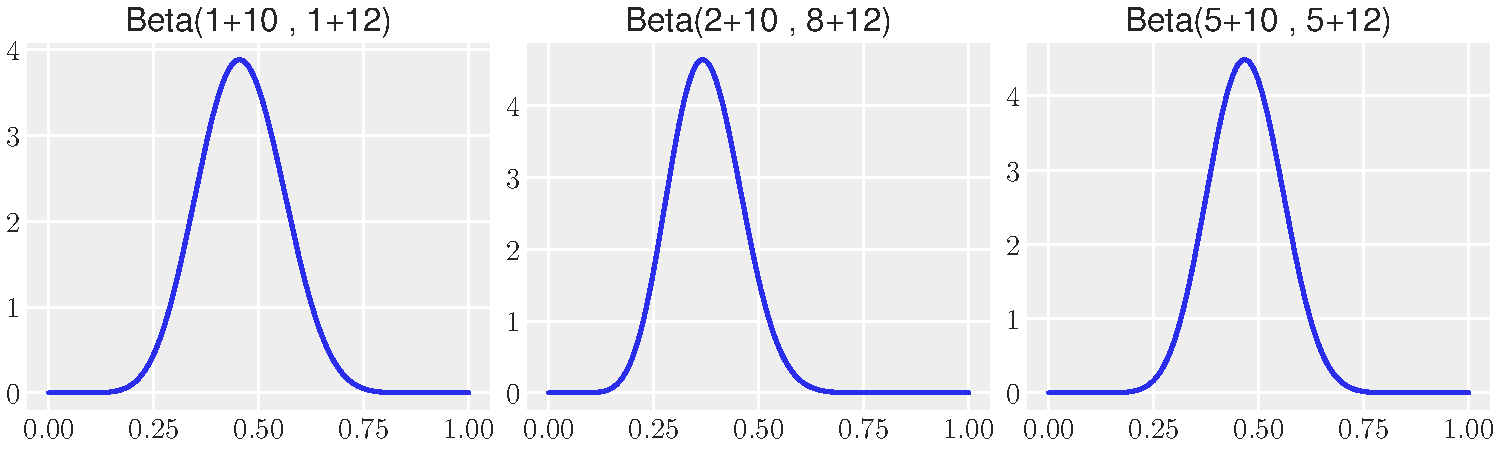
\includegraphics{3-coinTossing_files/figure-beamer/unnamed-chunk-11-5} \end{center}
\end{frame}

\begin{frame}{When the number of observations is large, the posterior is
the same whatever the prior}
\protect\hypertarget{when-the-number-of-observations-is-large-the-posterior-is-the-same-whatever-the-prior}{}
\begin{itemize}
\tightlist
\item
  The likelihood overwhelms the prior f
\end{itemize}

\begin{center}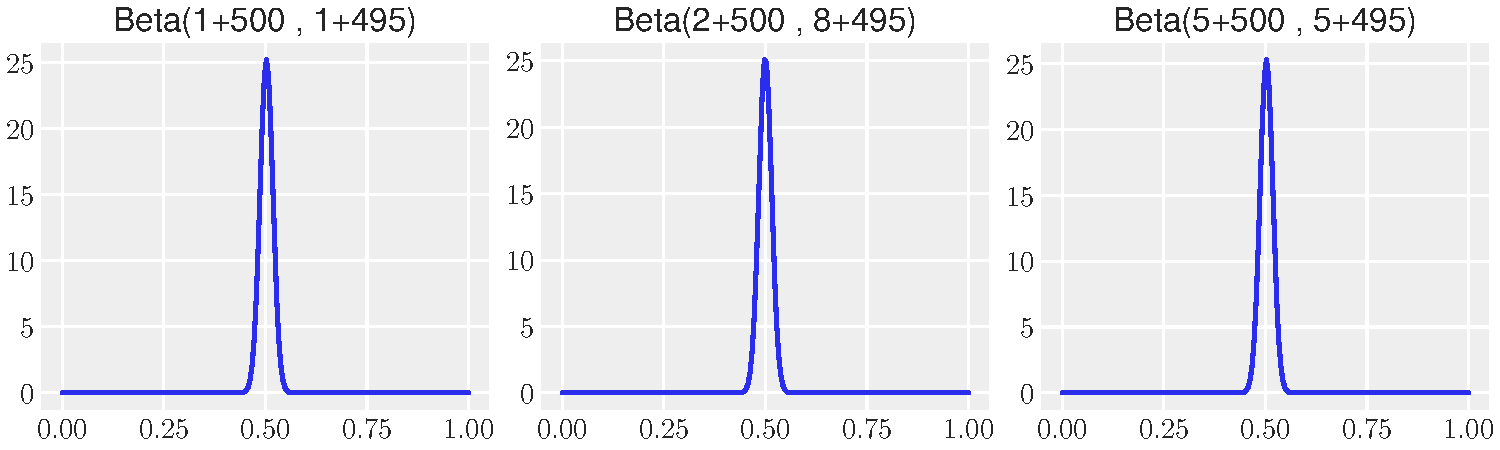
\includegraphics{3-coinTossing_files/figure-beamer/unnamed-chunk-12-7} \end{center}

The posterior means \(E_{\text{post}}[\theta]\) obtained using the
different priors are:

\begin{itemize}
\item
  \(\frac{500+1}{500+1+495+1}=\frac{501}{997}=0.502\)
\item
  \(\frac{500+2}{500+2+495+8}=\frac{502}{1005}=0.499\)
\item
  \(\frac{500+5}{500+5+495+5}=\frac{505}{1005}=0.502\)
\item
  Also the posterior variances and quantiles are practically identical
  in the different cases.
\item
  The likelihood \emph{overwhelms} the prior.
\end{itemize}
\end{frame}

\begin{frame}{The posterior mean is just part of the information}
\protect\hypertarget{the-posterior-mean-is-just-part-of-the-information}{}
\begin{itemize}
\item
  The result of the Bayesian analysis is the posterior distribution of
  \(\theta\), \textbf{not} a single value.
\item
  The dispersion of the posterior distribution (posterior variance) is a
  measure of our uncertainty.
\item
  The uncertainty decreases when the number of experiments is greater.
\item
  Given a large amount of data, the posterior is practically the same
  with any prior, but how much data is needed varies with the problem.
\item
  If we only have few data, the posterior can differ depending on the
  adopted prior; it makes sense to repeat the analysis with different
  priors (\emph{sensitivity}).
\item
  This is sensible: the prior encodes our previous knowledge and
  different experts could have different priors.
\end{itemize}
\end{frame}

\begin{frame}{Discussion}
\protect\hypertarget{discussion-1}{}
\begin{itemize}
\item
  Priors and likelihood are assumptions which are part of the model.
\item
  Uninformative priors (flat) provide the least possible amount of
  information and therefore have the least possible impact on the
  analysis.
\item
  \emph{Slightly informative} priors are recommended, which at least
  provide the order of magnitude of the parameter.
\item
  In many cases we known that the parameter can only be positive, or
  that they are restricted to sum to 1 or the approximate range, etc.
\item
  For instance even a Beta(1,1) prior is flat but limits the possible
  values of \(\theta\) between 0 and 1.
\end{itemize}
\end{frame}

\begin{frame}{Conclusions}
\protect\hypertarget{conclusions}{}
\begin{itemize}
\item
  We have seen how Bayesian inference works when Bayes' rule can be
  solved analytically, i.e., when the likelihood has a conjugate prior
  distribution.
\item
  In this case the posterior distribution has the same mathematical form
  as the prior.
\item
  Only simple likelihood functions have conjugate priors. In realistic
  applications the complex models have no conjugate priors. We will
  abandon exact mathematical solutions to use instead use numerical
  Markov chain Monte Carlo (MCMC) methods.
\end{itemize}
\end{frame}

\end{document}
